% === Fig. 2: Main Results ===
\begin{figure}[t]
    \centering
    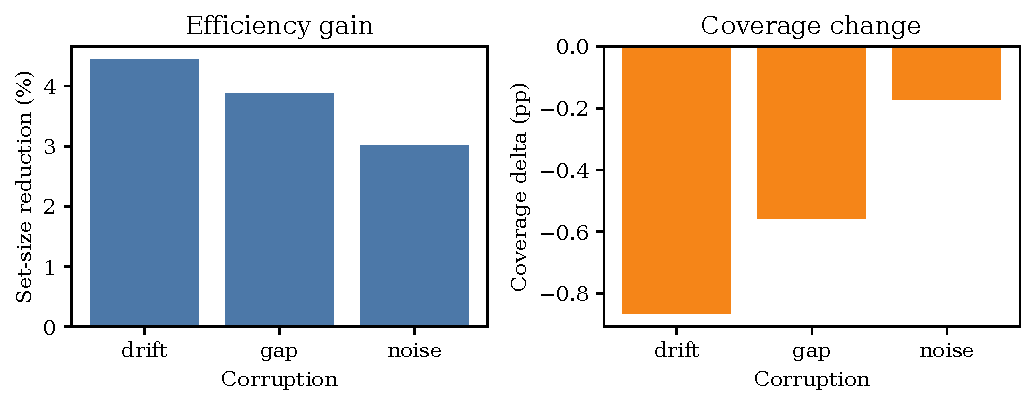
\includegraphics[width=0.95\linewidth]{figures/paper/fig2_main_results.pdf}
    \caption{Main 10-dataset, 3-seed results at $\alpha=0.05$. FAST-CP-mixed reduces prediction-set size relative to augmented split conformal prediction across drift, gap, and noise corruptions, with small coverage changes.}
    \label{fig:main_results}
\end{figure}

% === Fig. 3: Mix Ablation ===
\begin{figure}[t]
    \centering
    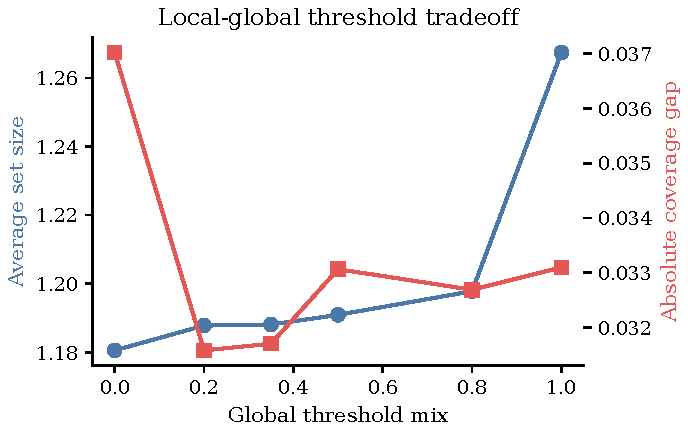
\includegraphics[width=0.58\linewidth]{figures/paper/fig3_mix_ablation.pdf}
    \caption{Ablation of the local-global threshold mix on five datasets. Intermediate mixing recovers coverage relative to purely local thresholds while retaining smaller prediction sets than the global augmented threshold.}
    \label{fig:mix_ablation}
\end{figure}

% === Fig. 4: Win/Loss Summary ===
\begin{figure}[t]
    \centering
    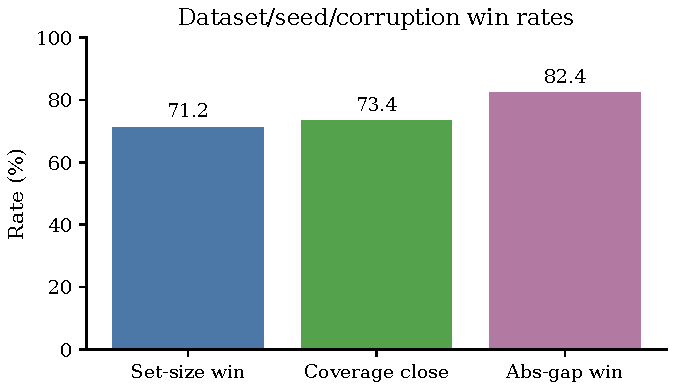
\includegraphics[width=0.58\linewidth]{figures/paper/fig4_win_loss.pdf}
    \caption{Dataset/seed/corruption-level comparison of FAST-CP-mixed against augmented split conformal prediction.}
    \label{fig:win_loss}
\end{figure}

% === Fig. 5: Runtime ===
\begin{figure}[t]
    \centering
    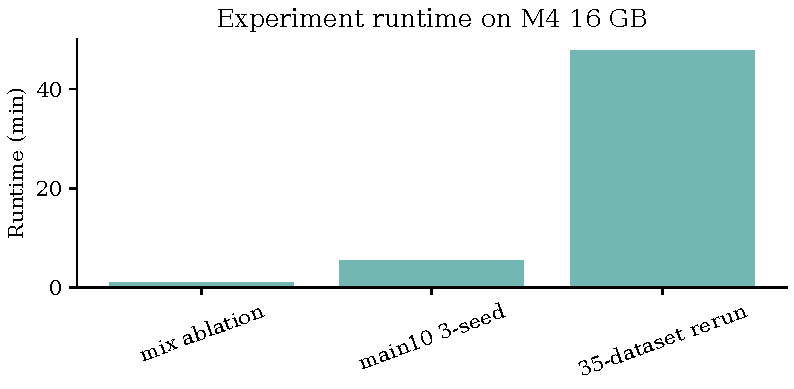
\includegraphics[width=0.62\linewidth]{figures/paper/fig5_runtime.pdf}
    \caption{Runtime of the main and ablation experiments on Apple M4 16 GB.}
    \label{fig:runtime}
\end{figure}
